\documentclass[a4paper]{report}
\usepackage{RJournal}
\usepackage[round]{natbib}
\bibliographystyle{abbrvnat}

%% load any required packages here

\begin{document}

%% do not edit, for illustration only
\fancyhf{}
\fancyhead[LO,RE]{\textsc{Contributed Article}}
\fancyhead[RO,LE]{\thepage}
\fancyfoot[L]{The R Journal Vol. X/Y, Month, Year}
\fancyfoot[R]{ISSN 2073-4859}

%% replace RJtemplate with your article
\begin{article}
%%%%%%%%%%%%%%%%%%%%%%%%%%%%%

\title{makeR: An R Package for Managing Document Building and Versioning}
\author{by Jason M. Bryer}

\maketitle

\abstract{
The idea of build automation is not new. \href{http://www.gnu.org/s/make/}{GNU Make} and \href{http://ant.apache.org}{Java Ant} are well established and robust build automation systems but require the use and installation of additional software. The \pkg{makeR} package provides a simplified framework written entirely in R to manage Sweave, \LaTeX{} and R scripted projects where multiple versions are created from a single source repository. For example, monthly reports where each version is identical, with perhaps the exception of easily extracted properties (e.g. date ranges for data extraction, title, etc.). 
}

R \citep{rcore}, \LaTeX{} \citep{latex}, and Sweave \citep{sweave} have proven to be incredibly useful for conducting reproducible research. However, managing document versions within R is limited. The \pkg{makeR} package attempts to provide the same ease-of-use for document versioning that the \pkg{devtools} \citep{devtools} and \pkg{ProjectTemplate} \citep{projecttemplate} packages have provided for package development and data analysis, respectively. This package attempts to solve the problem where multiple versions of a document are required but the underlying analysis and typesetting code remains static or can be abstracted through the use of variables or properties. For example, many researchers conduct monthly, quarterly, or annual reports where the only difference from version-to-version, from an analysis and typesetting perspective, is the data input. Clearly R and \LaTeX{} are an ideal solution to this problem. The \pkg{makeR} package provides a framework to automate the process of generating new documents from a single source repository.

\begin{figure*}
\vspace*{.1in}
\framebox[\textwidth]{\hfill \raisebox{0in}{\rule{0in}{0in}}
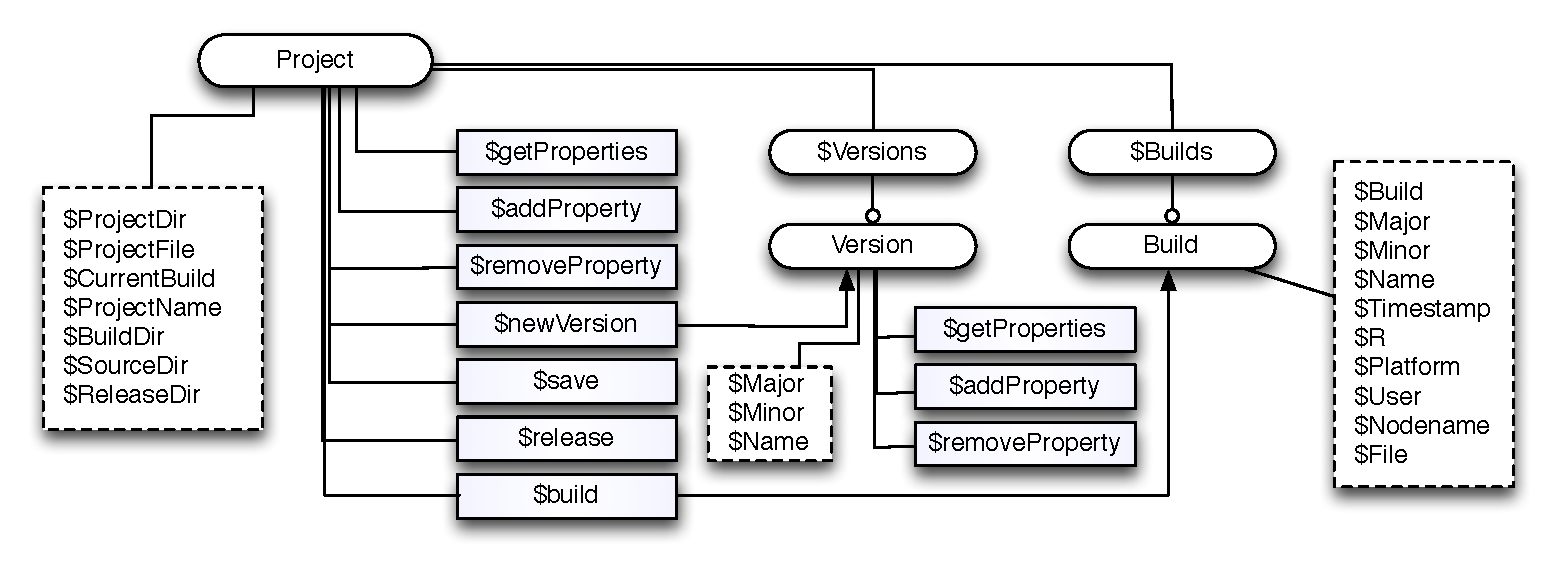
\includegraphics[width=\textwidth]{makeRClassDiagram.pdf}}
\caption{\label{figure:projectxml}\pkg{makeR} structure}
\end{figure*}

\section{Project framework}
There are three attributes to a particular document version: major (which can be numeric or character), minor, and build. Each major version is explicitly defined by the user. For example, if the goal of the project is to generate monthly reports then it would be appropriate to name each version using the month and year. Within each major version are minor versions. The minor version is always numeric and is incremented automatically upon each release. Lastly, build is numerical and global to the project that is automatically incremented with each document build. This index provides a unique identifier for each document that is created separate from the major and minor version identifiers.

From the perspective of the file system, the \pkg{makeR} package maintains a project file, \file{PROJECT.xml} (this will be discussed in further detail below), and three directories, \file{source}, \file{build}, and \file{release}. The \file{source} directory should contain all source files (typically a \file{.Rnw} file) along with any support files. The entire contents of this directory, including any subdirectories, will be copied for each build. \pkg{makeR} will create a new subdirectory in \file{builds} for each unique major and minor combination. Lastly, the \file{release} directory will contain ``released" documents (e.g. final PDFs). The \code{releaseVersion} function will rename build files to include the major and minor versions.

Consider, for example, a new project that contains a file \file{Example.Rnw} in the \file{source} directory. Each call of the \code{build} function will copy all files from the \file{source} directory to the \file{builds/1.0} directory, then call \code{Stangle}, \code{Sweave}, and \code{texi2pdf} to create \file{builds/1.0/Example.pdf}. Calling \code{release} will copy \file{bulids/1.0/Example.pdf} to \file{release/Example-1.0.pdf} and then increment the minor version so that subsequent calls to \code{build} will create the \file{builds/1.1} directory.

\section{Properties}
Properties are what differentiate one version from another and can be defined at the project or version level. When \pkg{makeR} builds a document project level properties will be assigned before version level properties thereby giving version level properties priority over project level properties. The functions \code{addProperty} and \code{removeProperty} for the objects of class type \code{Project} or \code{Version} (e.g. \code{myproject\$addProperty}, \code{myproject\$Versions[1]\$addProperty}) provide an interface for manipulating properties. 

\section{Package framework}
Figure \ref{figure:projectxml} represents the internal structure of a \pkg{makeR} project. All interaction with a project will occur through the \code{Project} class object. By convention, all attributes of classes begin with a capital letter and are represented in the boxes with dashed lined borders. Functions (or methods) begin with a lowercase letter and are represented in shaded boxes. Class objects and lists are represented by rounded squares. Project, Version, and Build are special classes for \pkg{makeR} whereas Versions and Builds are simply R lists. All manipulation of a project should be done through the appropriate methods. Although the attributes (i.e. elements of a list or class) are accessible given R's programming framework, doing so could result in unexpected results. The following two sections list the available attributes and methods.

\subsection{Project attributes}
\begin{itemize}
	\item \code{BuildDir} - the directory where builds will occur.
	\item \code{Builds} - list of completed builds. Each element in the list has a class type of \code{Build}.
	\item \code{CurrentBuild} - an integer of the last build.
	\item \code{ProjectDir} - the base directory where the project is located.
	\item \code{ProjectFile} - the name of the source file to be built.
	\item \code{ProjectName} - the name of the project.
	\item \code{ReleaseDir} - the directory where released files will be located.
	\item \code{SourceDir} - the directory containing the source files.
	\item \code{Versions} - a list of the project versions. Each element in the list has a class type of \code{Version}.
\end{itemize}

\subsection{Project methods}
\begin{itemize}
	\item \code{build} Builds the project.
		\begin{itemize}
		\item \code{version} - (optional) the version to build.
		\item \code{saveEnv} - if TRUE, the build environment (.rda) will be saved in the build directory.
		\item \code{builder} - the builder function.
		\item \code{clean} - if TRUE, a clean build will be performed (i.e. all files in the build directory will be deleted).
		\end{itemize}
	\item \code{rebuild} Rebuilds the project without first copying the files.
		\begin{itemize}
		\item \code{version} - (optional) the version to rebuild.
		\item \code{saveEnv} - if TRUE, the build environment (.rda) will be saved in the build directory.
		\item \code{builder} - the bulder function.
		\end{itemize}
	\item \code{save} Saves the PROJECT.xml file.
	\item \code{newVersion} Creates a new versions of the project.
		\begin{itemize}
		\item \code{name} - (optional) the version name.
		\item \code{properties} - version specific properties.
		\end{itemize}
	\item \code{release} Releases a version (i.e. copies the built file to the releases directory)
		\begin{itemize}
		\item \code{version} - (optional) the version to release. If omitted the latest version will be released.
		\end{itemize}
	\item \code{getProperties} Returns the project properties.
	\item \code{addProperty} Adds a project property.
		\begin{itemize}
		\item \code{name} - The property name.
		\item \code{value} - The property value.
		\end{itemize}
	\item \code{removeProperty} Removes the given project property.
		\begin{itemize}
		\item \code{name} - The property name.
		\end{itemize}
	\item \code{getReleases} Returns a list of released files.
	\item \code{openRelease} Opens the given released file with the system's default application.
		\begin{itemize}
		\item \code{file} - The released file to open.
		\end{itemize}
\end{itemize}

\section{The project file format}
\label{section:fileformat}

The \file{PROJECT.xml} file provides an XML formatted file corresponding to a project allowing for a project to persist across R sessions. The file is created and edited using the \pkg{XML} \citep{xml} package. Although the \pkg{makeR} package provides functions to manage projects, using XML allows for other R programmers to interact with the \pkg{makeR} project framework. Figure \ref{figure:projectxml} represents the contents of \file{PROJECT.xml} after running \code{demo('stocks')}.

\begin{figure*}
\vspace*{.1in}
%\framebox[\textwidth]{\hfill \raisebox{-.45in}{\rule{0in}{1in}}
\begin{example} 
<?xml version="1.0"?>
<project name="stocks" buildDir="build" releaseDir="release" sourceDir="source">
  <property name="src" type="character">
    <value>yahoo</value>
  </property>
  <property name="stocks" type="character">
    <value>GOOG</value>
    <value>AAPL</value>
    <value>AMZN</value>
    <value>MSFT</value>
  </property>
  <versions>
    <version name="2011-12" major="1" minor="1">
      <property name="month" type="character">
        <value>2011-12</value>
      </property>
    </version>
  </versions>
  <builds>
    <build major="1" minor="0" build="1" name="2011-12" timestamp="Thu Jan 26 20:55:10 2012" 
      R="R version 2.14.0 (2011-10-31)" platform="x86_64-apple-darwin9.8.0" 
      nodename="Jason-Bryers-MacBook-Air-2.local" user="jbryer">
      <file>2011-12.png</file>
    </build>
  </builds>
</project>
\end{example}
%}
\caption{\label{figure:projectxml}
\file{PROJECT.xml} for the stocks demo.}
\end{figure*}

\section{Example}

The \href{http://www.r-bloggers.com}{R-Bloggers} site provides a wealth of information about R and the R community, aggregated from many different R bloggers. Like many continuously changing data sources, we wish to periodically report on recent activity on the R-Bloggers site. The base source file, \file{rbloggers.Rnw}, is included in the package (in the \file{inst/doc/robloggers} directory) as well as being hosted on \href{https://github.com/jbryer/makeR/blob/master/inst/rbloggers/rbloggers.Rnw}{Github}. This example can also be run using \code{demo('rbloggers')}.

\subsection{Create new project}
The \code{Project} function will either create a new project or load a project if one already exists in the given project directory (the current working directory if not specified). Note that if a project already exists in the given directory, all other parameters (e.g. \code{name}, \code{properties}, etc.) will be ignored.

\begin{example}
myProject = Project(name="RBloggers", 
  projectDir="~/rbloggers",
  properties=list(email=email, passwd=passwd))
\end{example}

\subsection{Create initial version}
The \code{Project\$newVersion} method will create a new version for the project. Version names are optional but is recommended. \pkg{makeR} will ensure there are no two versions with the same name but if the name is not provided a new version will be created with the next numerical value equal to the number of versions plus one.

\begin{example}
myProject$newVersion(name='2011-12', 
  properties=list(startDate='2011-12-01', 
  endDate='2011-12-31'))
\end{example}

\subsection{Building the document}
The \code{Project\$build} function will build the newest version. The \code{version} parameter will allow for building of older versions. Values of class type \code{character} will build a version with a matching name, values of class type \code{numeric} will build the version corresponding the order in which it was created.

\begin{example}
myProject$build()
\end{example}

\subsection{Releasing the document}
Lastly, the \code{Project\$release} method will release the last built file(s). From a file system perspective, this method will copy the last built file to the release directory (as specified by the \code{Project\$ReleaseDir} attribute). Internally, the minor version number will be incremented so that any subsequent builds for this version will be done in a new directory. Similarly to the \code{Project\$build} method, a \code{version} parameter can be specified to release an older version.

\begin{example}
myProject$release()
\end{example}

\begin{figure}
\vspace*{.1in}
\framebox[\textwidth]{\raisebox{0in}{\rule{0in}{1in}}%
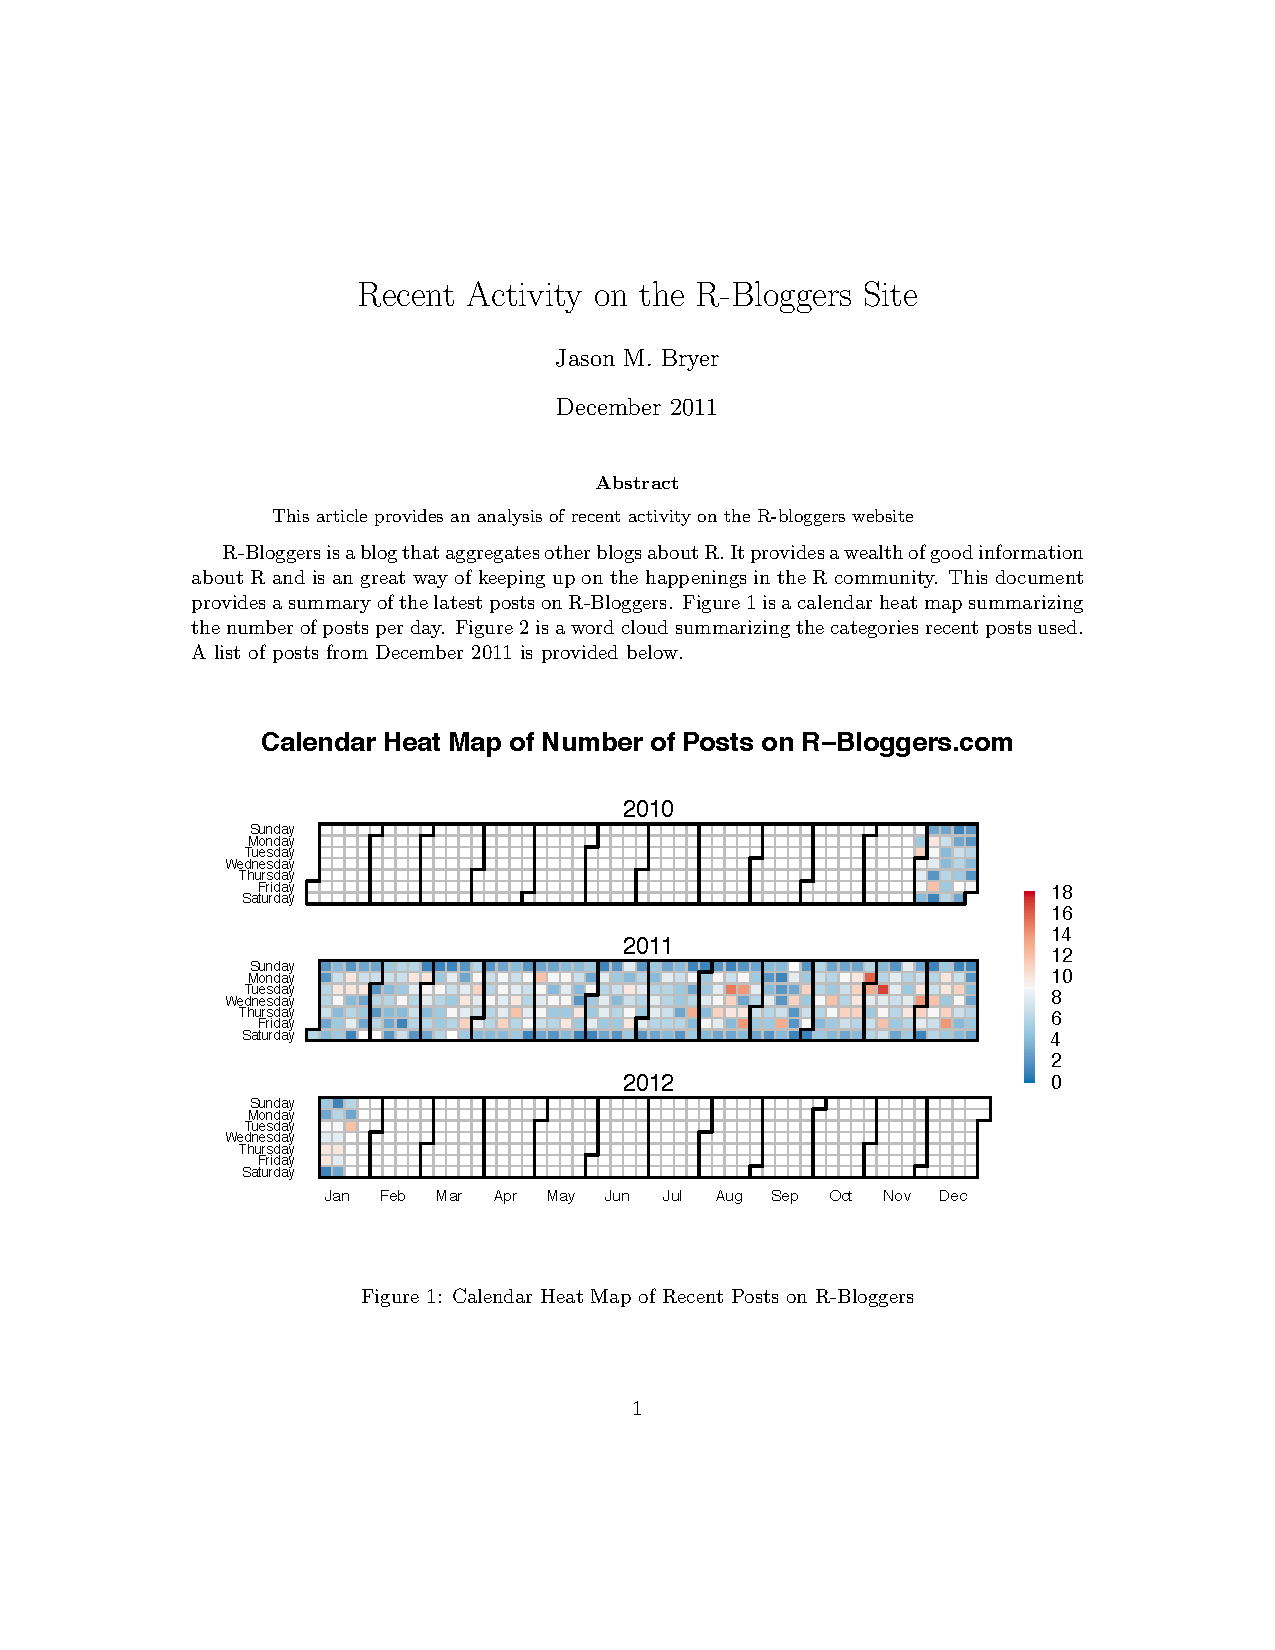
\includegraphics[width=\textwidth,trim=1cm 4cm 1cm 3cm,clip=true]{rbloggers.pdf}}%
\caption{\label{figure:rbloggers}%
Output from the R-Bloggers demo.}%
\end{figure}


\section{Builders}
The \pkg{makeR} package includes a number of builders for various document types. The default builder is \code{builder.rnw} but can be overwritten for your environment using the \code{setDefaultBuilder} function or by specifying the \code{builder} parameter to the \code{Project\$build} method. The included builders are:
\begin{itemize}
	\item \code{builder.rnw} used for building Sweave (.rnw) files.
	\item \code{builder.tex} used for building \LaTeX{} (.tex) files.
	\item \code{builder.cacheSweave} is similar to Sweave expect will support the \pkg{cacheSweave} \citep{cacheSweave} package and the caching of R code chunks.
	\item \code{builder.knitr} Uses the \pkg{knitr} \citep{knitr} package for building. This new package provides options for many other output types in addition to PDFs using \LaTeX{} including HTML and markdown. The default behavior for this builder is to look for Sweave (.rnw) files and process them using the \code{knit} function. To use other file types it is important to specify the \code{Project\$SourceFile} attribute and the \code{output} parameter to the \code{Project\$build} method. Otherwise the builder will not be able to locate the appropriate files to build.
\end{itemize}
Though the \pkg{makeR} package includes builders for for the most common document types, it has been designed to be extensible. A builder function requires two parameters, \code{project} and \code{theenv}. The former is simply the \code{Project} that is currently being built. The latter is an R environment with all the appropriate properties set. Any other parameters are passed from the \code{Project\$build} function to the \code{builder}. The following function builds projects where the input is an arbitrary R script file and the output are PNG image files. 

\begin{example}
builder.png <- function(project, theenv, ...) \{
  sourceFile = ifelse(
     is.null(project$SourceFile), 
    '.r$', project$SourceFile)
  wd = eval(getwd(), envir=theenv)
  files = list.files(path=wd,
      pattern=sourceFile,
      ignore.case=TRUE)
  for(i in seq_len(length(files))) \{
    sys.source(files[i], envir=theenv)
  \}
  return(list.files(path=wd, pattern=".png$",
    ignore.case=TRUE))
\}
\end{example}

%\section{Summary}


\section{Debugging}
The \pkg{makeR} package provides a number of facilities to help debug errors in the build process. First, all output is redirected to a log file in the build directory. Secondly, the build process is done in a new R environment. This environment is also saved to the build directory regardless if the builder method returns successfully or not. Lastly, each \code{Version} class has a method \code{assignProperties} that will assign the project and version properties to the global environment so the the user's global environment matches the environment passed to the builder function.  


\section{Package development}
The latest stable version of \pkg{makeR} can be installed from your local CRAN server. Development versions are hosted on \href{http://github.com/jbryer/ProjectVersion}{Github}. The latest development version can be installed using the \pkg{devtools} \citep{devtools} package:

\begin{example}
install_github('makeR', 'jbryer')
\end{example}

\bibliography{Bibliography}

\address{Jason M. Bryer\\
  Excelsior College\\
  7 Columbia Circle\\
  Albany, NY 12203\\
  USA}\\
\email{jason@bryer.org}


%%%%%%%%%%%%%%%%%%%%%%%%%%%%%
\end{article}

\end{document}

